\RequirePackage{plautopatch,fix-cm}
\documentclass[uplatex,dvipdfmx,a4paper]{jsarticle}
\usepackage[haranoaji]{pxchfon}
\usepackage[T1]{fontenc}
\usepackage[utf8]{inputenc}
\usepackage{lmodern}
\usepackage[dvipdfmx]{graphicx,color}
\usepackage{amsmath,amssymb,bm,braket,mathtools,mathrsfs,empheq,times,caption,cite}
\usepackage[top=25truemm,bottom=25truemm,left=20truemm,right=20truemm]{geometry} %余白の設定
\usepackage{setspace}
% 全体の行間調整
\renewcommand{\baselinestretch}{0.85}
% 図の名前を変更
\renewcommand{\figurename}{図.}
% 表の名前を変更
\renewcommand{\tablename}{Table.}
% 参考文献の名前を変更
\renewcommand{\refname}{参考文献}
% 図と図の間のスペース
\setlength\floatsep{0truemm}
% 本文と図の間のスペース
\setlength\textfloatsep{1truemm}
% \setlength\textfloatsep{0truemm}
% 本文中の図のスペース
\setlength\intextsep{0pt}
% 図とキャプションの間のスペース
\setlength\abovecaptionskip{0truemm}
% 数式上下の空白設定
\abovedisplayskip=4pt
\belowdisplayskip=4pt
% \abovedisplayskip=0pt
% \belowdisplayskip=0pt

\newcommand{\tabref}[1]{Table~\ref{#1}}
\newcommand{\equref}[1]{式~(\ref{#1})}
\newcommand{\figref}[1]{図.~\ref{#1}}

\usepackage{tcolorbox}
\usepackage{titlesec}

\titleformat*{\section}{\large\bfseries}
\newcommand{\red}[1]{\textcolor{red}{#1}}
\newcommand{\polylog}{\operatorname{polylog}}
\newcommand{\diag}{\operatorname{diag}}
% \everymath{\displaystyle} %数式を常にディスプレイスタイルにする

% sectionの前後の余白を詰める
\makeatletter
\renewcommand{\section}{%
    \@startsection{section}{1}{\z@}%
    {0.3\Cvs}{0.3\Cvs}%
    {\normalfont\normalsize\headfont\raggedright}%
}
\makeatother
% subsectionの前後の余白を詰める
\makeatletter
\renewcommand{\subsection}{%
    \@startsection{subsection}{1}{\z@}%
    {0.3\Cvs}{0.3\Cvs}%
    {\normalfont\normalsize\headfont\raggedright}%
    % {\normalfont\large\headfont\raggedright}%
}
\makeatother
% subsubsectionの前後の余白を詰める
\makeatletter
\renewcommand{\subsubsection}{%
    \@startsection{subsubsection}{1}{\z@}%
    {.25\Cvs}%
    {.25\Cvs}%
    {\headfont}
}
\makeatother

% 参考　http://www.ice.is.kit.ac.jp/~umehara/misc/comp/latex.html
\renewcommand{\topfraction}{1.2} %図表がページ上部を占める割合の上限
\renewcommand{\bottomfraction}{1.0} %図表がページ下部を占める割合の上限
\renewcommand{\dbltopfraction}{1.0} %二段組のとき段抜き図表がページ上部を占める割合の上限
\renewcommand{\textfraction}{0.01} % 文章がページを占める割合の下限
\renewcommand{\floatpagefraction}{1.0} % 図表がページを占める割合の上限
\renewcommand{\dblfloatpagefraction}{1.0} %二段組のとき段抜き図表がページを占める割合の上限
\setcounter{topnumber}{10} %ページ上部を占める図表の数の上限
\setcounter{bottomnumber}{10} %ページ下部を占める図表の数の上限
\setcounter{totalnumber}{20} %ページを占める図表の数の上限

\usepackage{url}
\usepackage[breaklinks=false,bookmarksnumbered=true,dvipdfmx]{hyperref} %ハイパーリンク
% \hypersetup{%
% bookmarksdepth=4,%
% bookmarksnumbered=true,%
% colorlinks=false,%
% urlcolor=magenta,%
% citecolor=green,%
% linkcolor=red,} %リンクの色
% 印刷時
\hypersetup{%
bookmarksdepth=4,%
bookmarksnumbered=true,%
colorlinks=true,%
urlcolor=black,%
citecolor=black,%
linkcolor=black,} %リンクの色


\begin{document}
\twocolumn[
\the\year 年度春合宿研究要旨
\hfill 指導教員 : 村松 眞由 准教授\\
\begin{spacing}{0.1}
  \centering
  \textbf{\large 研究タイトル}
\end{spacing}
\begin{flushright}
    村松研究室 学籍番号 氏名 
  \end{flushright}
]

\section{はじめに}
本稿では，春合宿研究要旨のテンプレートおよび\LaTeX を用いた文書作成における注意点を提供する．
本来の研究要旨であれば章立ては，1. 序論，2. 理論，3. 手法，4. 結果および考察，5. 結論のような構成が望ましい．
しかし，今回は研究要旨のテンプレートであるため，章立ては，1. 研究背景・目的，2. 理論，3. 方法，4. 今後の予定のような構成とする．
過去の春合宿の研究要旨は，Google Drive のMMC/03\_春合宿/アブストラクト例に保存されている．

\section{表記法}
物理量は，イタリック体 (斜体) で表記し，それ以外の単位等の文字はローマン体 (立体) で表記する．
また，スカラーは，$a$のように表記し，1階のテンソル (ベクトル) は$\bm{a}$のように太字小文字で表記し，2階のテンソルは，$\bm{A}$のように太字大文字で表記し，4階のテンソルは$\mathbb{A}$のように表記することが多い．
また，物理量の単位は，$1~\mathrm{m/s}$もしくは$a~[\mathrm{m/s}]$のように表記する．

\section{\LaTeX での注意点}
\subsection{数式周りの注意点}
文中で数式を入れるときには，$E=mc^2$というように書く．
また，式中で現れる変数や関数は全て説明する必要があり，例えば，$E$はエネルギー，$m$は質量，$c$は光速である．
さらに，式を別行にして書くときには，
\begin{equation}
    E = mc^2
    \label{eq:einstein}
\end{equation}
のように書き，式が文から独立しないようにする必要がある．
なお，連立方程式を書く場合には，
\begin{equation}
    \left\{
    \begin{aligned}
        x + y &= 1 \\
        2x - y &= 3
    \end{aligned}
    \right.
\end{equation}
のように書くと余白がいい感じになる気がする．
参照する場合には，式\eqref{eq:einstein}もしくは\equref{eq:einstein}のように書く．
また，分数をかっこで括る場合には，
\begin{equation}
    \left(\frac{a}{b}\right)
\end{equation}
と書くと括弧のサイズが自動的に調整される．
他にも数式周りで注意すべき点があるが詳細は，文献\cite{birdwatcher2019latex}を参照されたい．

\subsection{画像挿入の注意点}
画像には大きく分けてベクタ画像とラスタ画像の2種類がある．
ベクタ画像の代表例は，.pdfや.svgなどであり，点や線などの幾何学的な要素を数式で表現する画像形式である．
一方，ラスタ画像は，.pngや.jpgなどであり，ピクセルの集合で表現される画像形式である．
ベクタ画像は，拡大しても画質が劣化しないという特徴がある．
一方，ラスタ画像は，拡大すると画質が劣化するという特徴がある．
したがって，論文においてはグラフを挿入することが基本であるため，ベクタ画像を使用することが望ましい．
図\ref{fig:sin-pdf}はベクタ画像(PDF)の場合のグラフである．
一方，図\ref{fig:sin-png}はラスタ画像(PNG)の場合のグラフである．
図\ref{fig:sin-pdf}と図\ref{fig:sin-png}を比較すると，図\ref{fig:sin-pdf}の方が拡大しても画質が劣化しないことがわかる．
詳細の部分は文献\cite{tksmatsubara2022}を参照されたい．

\begin{figure}[t]
    \centering
    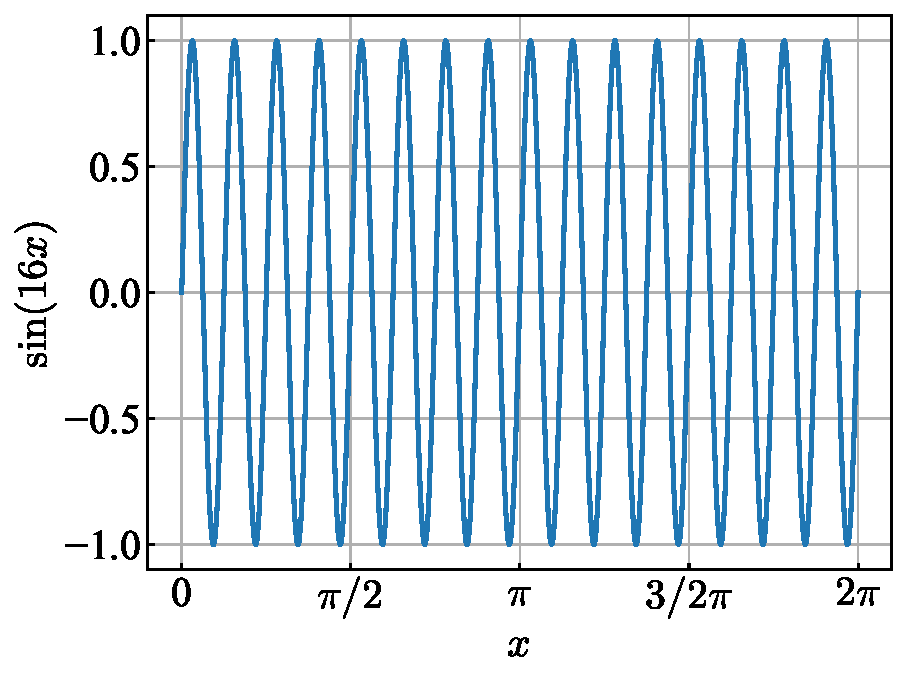
\includegraphics[width=\linewidth]{source/sin.pdf}
    \caption{ベクタ画像(PDF)の場合}
    \label{fig:sin-pdf}
\end{figure}

\begin{figure}[t]
    \centering
    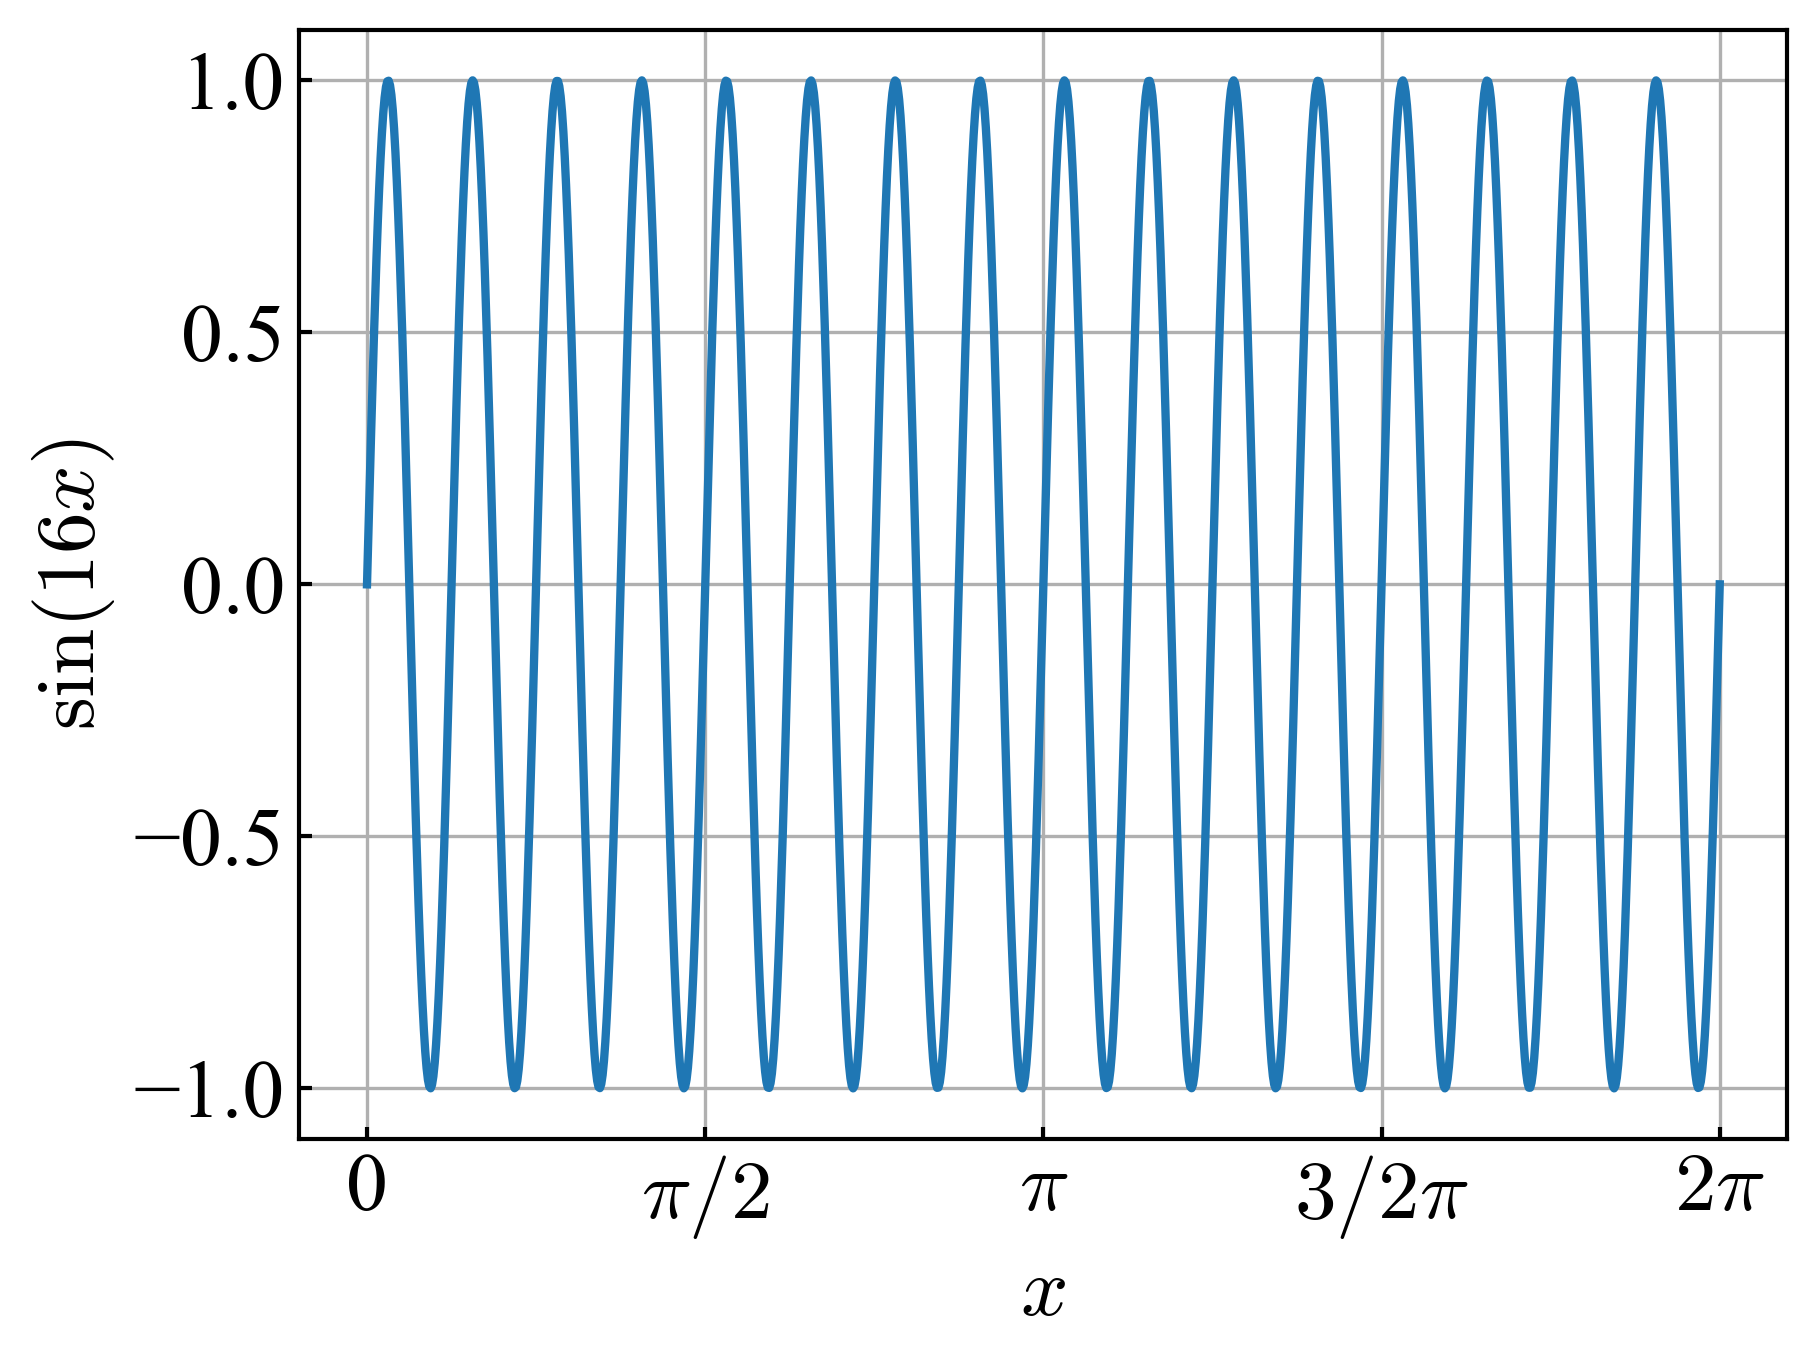
\includegraphics[width=\linewidth]{source/sin.png}
    \caption{ラスタ画像(PNG)の場合}
    \label{fig:sin-png}
\end{figure}

\subsection{参考文献の注意点}
先行研究を引用する際には，「村松ら\cite{muramatsu2014}は，核生成と核成長を同時に予測する静的再結晶の計算手法を提案した．」のように書くことが望ましい．
このように引用する際には，bibtexを使用して管理することが一般的であるがその利用方法に関しては，紙面の都合上割愛する．

\section{おわりに}
本稿では，春合宿研究要旨のテンプレートおよび\LaTeX を用いた文書作成における注意点を提供した．
紙面の都合上，詳細な説明を割愛した部分が多いため適宜調べてみたり，先輩に聞いてみるといいと思います．


\bibliographystyle{unsrt}
\bibliography{references}
\end{document}